\section{Literature Review}
% Answer research questions

\subsection{The need for Distributed Machine Learning}
.
\subsubsection{Alternatives to Distributed machine learning}
The most popular solution to increasing computation power for Machine
learning is currently distributing the workload over a large amount of machines. However, there are other, more traditional ways to increase the available computation power. Such as the use of dedicated Graphics processing units (GPUs), the use of Application Specific Integrated Circuits (ASICs) or special multi-core computer architectures.

\paragraph{GPUs in Machine Learning}
The use of GPUs in machinlearning is already a very common method. This is due to the nature of the data which makes up machine learning problems. A GPU is extremly fast at making multiple small calculations on a batch of data. Luckily the data that is requiered by Machine Learning algorithms such as Neural Networks and Unsupervised Learnign is of this type. This means that GPUs have had alot of succes with speeding up these calcultions as was found by Meuth \ref{Meut2007} who reported a up to 200x speed up over conventional CPUs.


\paragraph{Application Specific Integrated Circuits}
The idea of using Application Specific Integrated Circuits (ASICs) in highly specialized tasks is not new to Machine Learning. In recent times, the demand for such chips has risen massively\cite{Metz18}.
When applied to e.g. Bitcoin mining, ASICs have a significant competitive advantage over GPUs and CPUs, which achieve only a fraction of the performance per watt. The expectations of ASICs are high in the context of Machine Learning as well, because many of the computations involved come in the form of matrix multiplications. This is an area in which some ASICs excel.

Google applied this concept in their own Tensor Processing Unit (TPU)\cite{Sato17}, which, as the name suggests, is an ASIC that specializes in calculations that use tensors ($n$-dimensional arrays). The TPU works well when combined with their Tensorflow\cite{Tensorflow2015}\cite{Tensorflow2016} framework, which is one of the most popular building blocks for Machine Learning models.

The most important component of the TPU is its Matrix Multiply unit, which is what differentiates the chip from a CPU/GPU. The TPU can be connected to a server over a PCI-e bus. Many TPUs can be used in a data center, and if the work load is high even for a TPU, multiple units can collaborate in a distributed setting.

The performance improvement of the TPU over regular CPU/GPU setups is not only because of its increased processing power, but also its power efficiency, which is important for large companies that want to minimize energy costs. When running benchmarks, \citet{Joup17} found that the performance per watt of a TPU can approach 200x that of a traditional system.

Further benchmarking by \citet{Sato17} indicated that the total processing power of a TPU or GPU can be up to 70x higher than a CPU in a standard Neural Network, with performance improvements varying from 3.5x - 71x depending on the task at hand.


\paragraph{Computer architectures}
Other than using ASICs in order to increase the amount of work a computer can do,
general-purpose processors can also be built with different architectures that significantly increase the number of usable cores. Such an architecture exists in the form of Epiphany. It is a Multiple Instruction, Multiple Data (MIMD) architecture that uses an array of processors, each of which accessing the
same memory, to speed up execution of floating point operations\cite{Olof16}.

The newest chip of the major manufacturer Adapteva is the Epiphany V, which contains
1024 cores on a single chip\cite{Olof16}. Although Adapteva has not published power consumption specifications of the Epiphany V yet, it has released numbers boasting a power usage of only 2 watt\cite{Adap}.

Using multiple processors to process a single dataset is not a new idea in Computer Science. Message Passing Interface (MPI)\cite{MPI1993} was developed to simplify the distribution of work for this purpose, and is usually applied on a cluster of workers. The same framework, however, can also be adapted to the Epiphany chips, as was demonstrated by \citep{Rich15}. They found that the RISC chips were able to perform matrix operations rapidly until their on-board memory was filled.

\paragraph{Future relevance}
As can be seen in the examples above, there are many different strategies to obtain the processing power needed for large-scale Machine Learning. These techniques focus both on power efficiency and raw computational power. However, it must be noted that distributed systems are often preferred to these non-distributed alternatives above a certain scale, because of higher scalability and lower equipment cost. The techniques described above can still be used in a distributed setting, without suffering major performance degradations. This makes them a good choice for certain classes of future applications, as they can provide the benefits of optimized hardware in a distributed system.










\subsection{Underlying technology}
To give you an overview of how Distributed Machine Learning works, we'll give you an abstract framework that includes everything a real implementation should include. We do that by exploiting the three unique properties of Distributed Machine Learning, namely error tolerance, dynamic structural dependency and non-uniform convergence.\cite{Xing16}\\
Our goals include (1) to list regular Machine Learning algorithms that are commonly used in a distributed setting; (2) to find algorithms to determine the best parameters for the former algorithms; (3) to tradeoff computation time with communication and accuracy; and (4) to minimize the amount of bits sent over the network so that the system is no bottlenecked by scarce network bandwidth.\\
Designing a general system in such a way that the regular Machine Learning algorithms can be distributed efficiently is challenging, because every algorithm has its own communication patterns \cite{Jia14}\cite{Newman09}\cite{Rich13}\cite{Smola10}\cite{Takac13}\cite{Tsi12}.

\subsubsection{Machine Learning algorithms}
Machine learning algorithms learn to make predictions or decisions based on data. Every machine learning algorithm has its own pros and cons. Machine learning algorithms can be divided into categories based on some of their characteristics;
\begin{itemize}
	\item \textbf{Feedback}, the type of feedback given to the algorithm during its learning
	\item \textbf{Goal}, the type of output
	\item \textbf{Type}, the way they create their output
	\item \textbf{Method}, the way they change when given feedback
\end{itemize}

\paragraph{Feedback}
\begin{itemize}
	\item \textbf{Supervised}
		learning uses training data which consists of input objects, usually vectors, and output values. Supervised learning algorithms typically try to find a function to map input to output and use that to find outputs for unknown input objects.
		% bias vs variance
		% complexity vs amount of data
		% dimensionality
		% noise
	\item \textbf{Unsupervised}
		learning uses training data without labels, which means there is no way to look at the accuracy of the output. It is more commonly used to find clusters of datapoints or patterns.
	\item \textbf{Semi-supervised}
		learning make use of a usually small amount of labeled data and a large amount of unlabeled data. Clustering can be used to extend the labels known to other datapoints. This is done under the assumption that similar datapoints share a label.
	\item \textbf{Reinforcement learning}
		is done by having the model generate an output and having a different system give feedback on how well the output matches the desired output. This is done by either minimizing a risk function or by maximizing a reward function. This means that reinforcement learning can be done without having a big dataset of correct and incorrect input-output pairs. Because of the black box behavior of the model, it is not possible to explicitly correct actions that are sub-optimal and the model might get stuck in a local minimum.
		% Q-learning
\end{itemize}

\paragraph{Goals}
\begin{itemize}
	\item \textbf{Anomaly detection}
		can be divided into three categories. \textbf{Supervised anomaly detection} requires data that has a different label for abnormal data and trains a normal classifier. \textbf{Unsupervised anomaly detection} assumes that normal and abnormal datapoints will be groups separately and effectively does clustering. \textbf{Semi-supervised anomaly detection} builds a model of normal data and test whether new datapoints are normal or abnormal. Based on the dataset, different methods perform better than others
	\item \textbf{Classification}
		is the problem of putting new datapoints in categories based on the categories of the training data. This is an inherently supervised process. The unsupervised version of this is Clustering.
	\item \textbf{Clustering}
		is the problem of grouping together datapoints that are similar according to some criteria. This can be done supervised, but is usually done with significantly big datasets for which labeling might be too expensive
	\item \textbf{Dimensional reduction}
		is the problem of reducing the amount of variables looked. This can be done by either selecting only those variables that are relevant, called \textbf{Feature selection}, or by creating new variables that represent multiple other variables, called \textbf{Feature extraction}.
	\item \textbf{Feature learning / Representation learning}
		is the set of techniques designed for finding good representations of the data for things like feature detection, classification, clustering, encoding and even matrix factorization.
		% manifold learning
		% statistical inference/density estimation
		% sparse coding
	\item \textbf{Regression}
		is the problem of estimating how a dependent variable changes with changes to the independent variables. Parametric regression tries to find the parameters of a function, which speeds up the process if for example a linear correlation is expected. Nonparametric regression also tries to find the type of function, but this requires a larger sample size and significantly more time.
\end{itemize}

\paragraph{Types}
\begin{itemize}
	\item \textbf{Evolutionary algorithms (EAs)},
		specifically \textbf{Genetic algorithms (GAs)} are algorithms that learn iteratively based on evolution. The algorithm that actually solves the problem is represented by a set of data that determine its properties, called its \textbf{genotype}. The performance of the algorithm is measured using an objective score, calculated using a \textbf{fitness function}. After calculating the fitness of all generated algorithms, the next iteration creates new genotypes based on mutation and crossover of algorithms that are 'more fit'. Generic algorithms can be used to create other algorithms like neural networks, belief networks, decision trees and rule sets.
	% Graphical models
	\item \textbf{Perceptron-based}
		algorithms are based on perceptrons, binary classifiers that map an input vector to being 'active' or 'inactive' by assigning a weight to all inputs and summing over the products of these weights and their inputs and comparing them to a threshold number, usually called the bias. Perceptron-based algorithms commonly use the entire batch of training data to try to find an instance that will work for the entire set. Perceptron-based algorithms are binary and are therefore mainly used binary or multi-label classification.
	\item \textbf{Rule-based machine learning (RBML)}
		algorithms use a set of rules that each represent a small part of the problem. These rules usually express a condition and a result for when that condition is met. Because of this if-then relation, rules lend themselves to be more easily interpreted than more abstract types of machine learning algorithms such as neural networks.
	\item \textbf{Topic Models (TM)}
		are statistical models for finding and mapping semantic structures in text.
\end{itemize}

\paragraph{Methods}
\begin{itemize}
	\item \textbf{Association rule learning}
		is a \textit{rule-based machine learning} method that focuses on finding relations between different variables in datasets. This is done by looking at some measure of interest. Examples of this are \textbf{Support}, how often variables appear together; \textbf{Confidence}, how often a causal rule is true; and \textbf{Collective Strength}, a comparison of the amount of instances which contains some but not all variables in the relation and the expected amount if the variables where not related.
	\item \textbf{Artificial neural networks (ANNs)}
		are perceptron-based systems using multiple layers. These layers are usually divided into an input layer, an output layer, and one or more hidden layers. Each layer consists of nodes connected to the previous and next layers by weights, usually called synapses. Unlike normal perceptrons, nodes usually use an activation function instead of just a bias.
		The workings of the algorithm is dependent on the entire network, the algorithm can be changed by changing (1) the weights of the synapses, (2) the layout of the network or (3) the activation function of nodes.
		Because neural networks require a big amount of nodes, the un-understandability of what a neural network actually does is a major drawback when comparing it to for example decision trees.
		Neural networks are extensively studied for their ability to analyze enormous sets of data. Neural networks can be divided into subgroups based on the layout of the network;
		\begin{itemize}
			\item \textbf{Recurrent neural networks (RNNs)}
				have synapses going back to previous layers, which means that the previous state of the network influences its current decisions. Neural networks that are not recurrent are called \textbf{feed-forward}. Recurrent synapses give the network a sort of memory that can help with discovering patterns in data that arrives sequentially. Special blocks of nodes in a network can work as a memory cell that can hold some information for an arbitrarily long timespan. These blocks are called long short-term memory (LSTM) units.
				% finite impulse
				% 	DAG which can become a feedforward network 
				% vs infinite impulse
				% 	DAG which can not be unrolled
			\item \textbf{Hopfield networks}
				are a type of non-reflexive, symmetric recurrent neural network that have some 'energy' related to every state of the network as a whole which will reach a local minimum after continuously updating the network.
			\item \textbf{Deep neural networks (DNNs)},
				opposite of \textbf{shallow neural networks}, have many hidden layers, which may cause the network to work as a sort of black box
			\item \textbf{Convolutional neural networkss (CNNs / ConvNets)}
				are deep, feed-forward neural networks that use convolution layers with nodes connected to only a few nodes in the previous layer. These values are then pooled using pooling layers that can be seen as a way of recognizing abstract features in the data. The convolution makes the network look at local data, making the entire algorithm spatially invariant, which is why they are sometimes called space invariant artificial neural networks (SIANN). Chaining multiple of these convolution and pooling layers together can make the network very good at recognizing complicated constructs in big datasets, like recognizing cars in images or the contextual meaning of a sentence in a paragraph.
			\item \textbf{Generative adversarial networks (GANs)}
				consist of two separate networks, one trying to recognize objects from a dataset and one trying to create new data in an attempt to 'fool' the other network into thinking the data is legit.\cite{Li:2013:CAL:2463372.2465801}
			\item \textbf{Radial Basis Function (RBF) networks}
				\cite{rbf}
			\item \textbf{Self-organizing maps (SOMs) / self-organizing feature maps (SOFMs)}
				are neural networks that learn by unsupervised \textbf{competitive learning}, in which nodes compete for access to specific inputs, causing the nodes to become highly specialized, which reduces redundancy. Iterations effectively move the map closer to the training data, which is where it gets its name from. Some subtypes include time adaptive self-organizing map (TASOM), Binary Tree TASOM (BTASOM) and growing self-organizing map (GSOM)
			\item \textbf{Stochastic neural networks}
				make use of stochastic transfer functions or weights, which makes it possible to escape a local minimum. 
			% 		boltzmann machine
		\end{itemize}
		Neural networks trained in many different ways, like using Generic algorithms. The most common approach, especially when talking about Deep neural networks, is using a process called \textbf{backpropagation};
		\begin{itemize}
			\item Present a training sample
			\item Calculate the error in each output neuron, how much lower or higher the output must be adjusted to match the desired output
			\item Calculate the gradient
			\item For every layer, adjust the weights and biases based on the gradient
			\item Repeat
		\end{itemize}
	\item \textbf{Autoencoders}
		are a type of neural network that trained specifically to encode and decode data. Because autoencoders are trained to also decode, the encoded version of the data can be seen as a dimensional reduction of the data
	\item \textbf{Bayesian networks}, 
		sometimes called \textbf{belief networks}, are probabilistic directed acyclic graphical models\cite{Wain08}\cite{Kol09}\cite{Xin16} that are used to represent conditional relationships between variables. They are directed to overcome the problems of \textbf{Markov random
		fields (MRFs)}, also called \textbf{Markov networks}, which use undirected connections. These undirected connections make it impossible to represent dependencies that are non-transitive or otherwise induced. Bayesian networks are commonly used to represent \textbf{Markov processes} (not related to Markov networks) in particular for probabilistic inference or parameter estimations.
		\textbf{Nonparametric Bayesian models}\cite{Grif05}\cite{Teh06} don't fix the parameters in place, allowing the model to grow with the data size.
	%		Regularized Bayesian models \cite{Zhu09}\cite{Zhu09-2}\cite{Zhu14}
	\item \textbf{Decision trees},
		sometimes called CART trees, after Classification And Regression Trees trees (RAS syndrome), use Rule-based machine learning to create a set of rules that create decision branches. Traversing the tree means applying the rules at each step till you arrive at a leaf of the tree, which represents the decision or classification for that input.
	\item \textbf{Latent Dirichlet Allocation}\cite{Blei03}
		makes a mapping between documents and probabilistic set of topics, using the assumption that documents have few different topics and topics use few different words.
	\item \textbf{Latent semantic analysis (LSA) / latent semantic indexing (LSI)}
		creates a big matrix of documents and topics in an attempt to classify documents or to find relations between topics. LSA/LSI assumes a Guassian distributes for topics and documents. LSA/LSI doesn't have a way of dealing with words that have multiple meanings.
	\item \textbf{Naive Bayes classifiers}
		are relatively simple probabilistic classifiers that assume different features are independent. They can be trained quickly using supervised learning, but are less accurate than more complicated approaches.
	\item \textbf{Probabilistic latent semantic analysis (PLSA) / probabilistic latent semantic indexing (PLSI)}
		is the same as LSA/LSI, except that PLSA/PLSI assumes a Poisson distributes for topics and documents instead of the Guassian distribution that is assumed by LSA/LSI, because the Poisson distribution appears to model the real world better. Some subtypes include Multinomial ASymmetric Hierarchical Analysis (MASHA), Hierarchical Probabilistic Latent Semantic Analysis (HPLSA) and Latent Dirichlet Allocation (LDA).
	% Inductive logic programming (ILP)
	\item \textbf{Support vector machines (SVMs)}
		map datapoints to high dimensional vectors for classification and clustering purposes. For datapoints in p-dimensional space, a (p-1)-dimensional hyperplane can be used as a classifier. A reasonable choice would be the hyperplane that properly separates the datapoints in two groups based on their labels, that also has the biggest possible margin. Sometimes special transformation equations, called \textbf{kernels}, are used to change all datapoints to a different representation in which it is easier to find such a hyperplane.
		Having a lot of dimensions decreases the accuracy of classifying new datapoints, so increasingly large datasets are needed to make the algorithms perform well
\end{itemize}

Usually a single algorithm isn't enough to solve a problem, and multiple algorithms are combined in something ofter called \textbf{Ensemble Learning}. There are many different ways to do this, depending on what kind of algorithms are used;

\begin{itemize}
	\item \textbf{Bagging}
		is the process of building multiple classifiers and combining them into one.
	\item \textbf{Boosting}
		is the process of training new models with the data that is misclassified by the previous models.
	\item \textbf{Bucketing}
		is the process of training many different models and eventually selecting the one that has the best performance.
	\item \textbf{Random Forests}\cite{Breiman2001}
		use multiple decision trees and averaging the prediction made by the individual trees as to increase the overall accuracy. Different trees are given the same 'voting power'.
	\item \textbf{Stacking}
		is when multiple classifiers are trained on the dataset and one new classifier uses the output of the other classifiers as input in an attempt to reduce the variance.
	\item \textbf{Learning Classifier Systems (LCSs)}
		(not to be confused with the more common usage of the LCS initialism, Longest Common Subsequence) is a kind of modular system of learning approaches. An LCS iterates over datapoints from the dataset and completes the entire learning process in each iteration. The main idea is that an LCS has a limited number of rules that are follow a Genetic Algorithm that forces rules that are suboptimal out of the ruleset. There are many different overall attributes that can drastically change the performance of the LCS based on the dataset;
		\begin{itemize}
			\item Michigan-style architecture vs Pittsburgh-style architecture
			\item supervised vs reinforcement
			\item incremental vs batch
			\item online vs offline
			\item strength-based vs accuracy-based
			\item complete mapping vs best mapping
		\end{itemize}
		Because of increasing complexity of the training of LCS with respect to the size of the data, LCS is mainly used 
\end{itemize}


%Deep learning
%
%Multi-task learning (MTL) 
%
%Matrix factorization
%Singular value decomposition (SVD) and principal component analysis (PCA)


\paragraph{Algorithms to find best parameters}
To find the parameters for these algorithms we can use several Machine Learning workhorse implementations that can be re-used across different Machine Learning algorithm-families. These include:
\begin{itemize}
	\item First-order techniques
	\begin{itemize}
		\item Stochastic gradient descent
% 			Backpropagation
		\item Stochastic dual coordinate ascent\cite{Shal13}
		\item L-BFGS
		\item Conjugate gradient
	\end{itemize}
	\item Second-order techniques
	\begin{itemize}
		\item Newton descent
		\item Quasi-Newton descent
	\end{itemize}
	\item Coordinate descent
	\item Markov-Chain Monte-Carlo
	\item Variational inference
\end{itemize}


% --------


\subsubsection{Partitioning and distribution algorithms}
Now we'll look the abstraction of the general design for a distributed Machine Learning operating system that executes the Machine Learning workhorses across a wide variety of hardware.


\paragraph{Computation time vs communication vs accuracy}


\paragraph{Scheduling and balancing the workloads}
There are 3 things to take into account when partitioning an ML program in order to parallelize it:\cite{Xing16}\\
\begin{enumerate}
	\item Deciding which tasks go or don' go together in parallel
	\item Deciding the order in which tasks will be executed
	\item Ensuring an even load distribution across the machines
\end{enumerate}


\paragraph{Bridging computation and communication}
Let's look at several ways to efficiently communicate between the nodes taking the interleaving of parallel program computations and inter-worker communication into account. These techniques tradeoff fast / correct model convergence (at the top of the list) with faster / fresher updates (at the bottom of the list).
\begin{enumerate}
	\item \underline{BSP:} Bulk Synchronous Parallel, the most simple model; programs will alternate between a computation and a communication phase to ensure consistency\cite{Xing16}. An example of program following the BSP bridging model is MapReduce.\\
	An advantage is that serializable BSP ML programs are guaranteed to output a correct solution. A disadvantage is that finished workers must wait at every synchronization barrier till the other works are finished, which results in overhead\cite{Chilimbi14}. Another disadvantage is that the synchronization barrier may take a significant amount of time, because of slow communication between the workers.
	\item \underline{SSP:} Stale Synchronous Parallel, allows the fastest worker to be ahead of the slowest worker up to a bounded number of iterations before the workers are stopped. The fast workers may work for a while on state data, but SSP still limits the maximum staleness between any pair of workers. An advantage is that it still enjoys strong model convergence guarantees. A disadvantage is that, when machines temporarily slow down due to other tasks or users and cause large staleness, the convergence rates are poor.
	\item \underline{ASP:} Approximate Synchronous Parallel, limits how inaccurate a parameter can be, in contrast to SSP that limits how stale a parameter can be. An advantage is that, when an aggregated update is insignificant, then the server can delay synchronization indefinitely. A disadvantage is that it can be hard to choose the parameter that defines which update are significant and which are not. \cite{Hsieh17}
	\item \underline{BAP / TAP:} Barrierless Asynchronous Parallel\cite{Han15} or Total Asynchronous Parallel\cite{Hsieh17}; worker machines communicate in parallel without waiting for each other. The advantage is that it usually obtains the highest speedup possible. A disadvantage is that the model converges slowly or even incorrectly because the error grows with the delay, unlike BSP and SSP. \cite{Han15}
\end{enumerate}
At the moment, ASP is the state-of-the-art method.


\paragraph{Communication strategies}
To distribute Machine Learning algorithms we can choose to partition either the data or the model across the machines - referred to respectively as data parallelism and model parallelism \cite{Die12}. These two types of parallelism can be applied at the same time \cite{Xing16}. Data parallelism can be applied to every ML algorithm with an i.i.d. assumption over the data samples, which are most ML algorithms \cite{Xing16}. It partitions the data and assigns it to parallel machines. Model parallelism cannot be applied to most ML algorithms, because the model parameters generally don't have this i.i.d. assumption. It partitions the model parameters and assigns that to parallel machines.\\
There are several communication management strategies\cite{Xing16} used to spread and reduce the amount of data communicated between machines:
\begin{itemize}
	\item To prevent bursts of communication over the network, for example after a mapper is finished, continuous communication is used, for example in the state-of-the-art implementation Bösen\cite{Wei15}.
	
	\item Neural networks are composed out of layers, of which the training by using the back-propagation gradient descent algorithm is highly sequential. Because the top layers of neural networks contain a lot more parameters while it accounts only for a small part of the total computation \cite{Xing16}, WFBP \cite{Zhang17} was proposed to spread the computation and communication out in an optimal fashion.
	
	\item Hybrid communication (HybComm) Because WBFP does not reduce the communication overhead, HybComm \cite{Zhang17} was proposed. Effectively it combines Parameter Servers (PS)\cite{Wei15} with Sufficient Factor Broadcasting (SFB)\cite{Xie15} by being aware of both the mathematical property of neural networks and the structure of computing clusters. See below for more information about PS under Centralized Storage and SFB under Decentralized Storage.
	
\end{itemize}


\paragraph{Network topologies}
There are several network topologies used for Distributed Machine Learning clusters:
\begin{itemize}
	\item \textbf{Trees} AllReduce\cite{Agar14} is an example of a tree-like network topology that provides straightforward parallelization of gradient-based optimization algorithms by accumulating local gradients to obtain a global gradient.\\
	An advantage is that AllReduce is very fast and highly scalable. A disadvantage is that it only works for reduce operations like in MapReduce.
	\begin{minipage}{\linewidth}
		\centering
		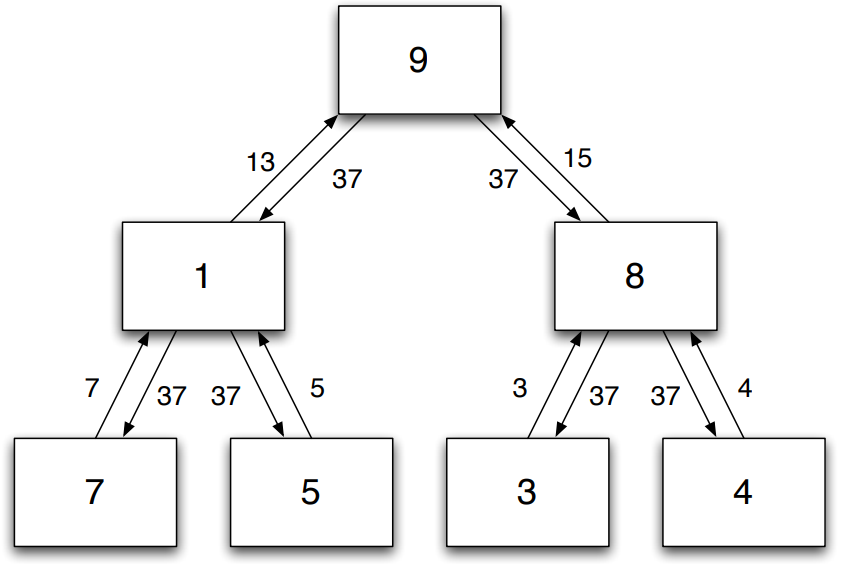
\includegraphics[scale=0.5]{AllReduce.png}
		\captionof{figure}{AllReduce operation. Initially, each node holds its own value. Values are passed up the tree and summed, until the global sum is obtained in the root node (reduce phase). The global sum is then passed back down to all other nodes (broadcast	phase). At the end, each node contains the global sum.}
	\end{minipage}
	\item \textbf{Centralized storage} Centralized storage is used for topologies where a single "master" or "server" node is in the center and many "slave" or "client" nodes communicate only with this master node. A practical implementation of this is the Parameter Server paradigm (PS). Each parameter server keeps a shard of the global model parameters as a key-value store. Each client communicates with the parameter server to read / update the parameters. \\
	An advantage is that all model parameters are in a global shared memory which makes it easy to inspect the model. A disadvantage is that the parameter servers are a bottleneck because they're handling all communication. To partly accommodate this issue, the techniques mentioned under "Bridging computation and communication" are used.
	\item \textbf{Decentralized storage} In contrast to centralized storage, in decentralized storage every worker maintains its own local view of the parameters and the workers communicate directly to each other. An example implementation is a peer-to-peer network where every machine broadcasts everything to all other machines. To reduce the amount of communication between all workers, Sufficient Factor Broadcasting (SFB)\cite{Li13}) was proposed. It decomposes the parameter matrix into so-called sufficient factors, i.e. 2 vectors that are sufficient to reconstruct the update matrix. SFB only broadcasts the sufficient factors and lets the workers reconstruct the updates.\\
	An advantage is that, with SFB, decentralized storage is relatively communication efficient and that there is no centralized bottleneck, making it more scalable.
\end{itemize}










\subsection{Currently used implementations}
\subsubsection{Generic distributed system frameworks}
Distributed system have already been implemented in the industry to solve the problem of companies possessing massive amounts of data that they want to be able to query and analyze. These frameworks largely rely on the fact that it is cheaper
to have multiple servers, each of them with a relatively small storage capacity and computing power, rather than having one expensive large server.

\paragraph{The frameworks}
The basis of existing frameworks is based on the Google File System\cite{Ghem03}. The \textit{Google File System} or \textit{GFS} is the system that is used within Google to handle all the Big data needs within the company. It splits all the data that is uploaded to the cluster up into chunks, which are then split over the "chunk servers" in the node, and replicated a predefined number of times (usually 3) in order to guarantee that the data is not lost when a server fails. The
data on the chunk servers can then be accessed by a user by contacting the master, which knows exactly on which servers each chunk is saved.\cite{Ghem03} The data and work-flow is described in figure \ref{GFS_Architecture} below.

\begin{figure}
  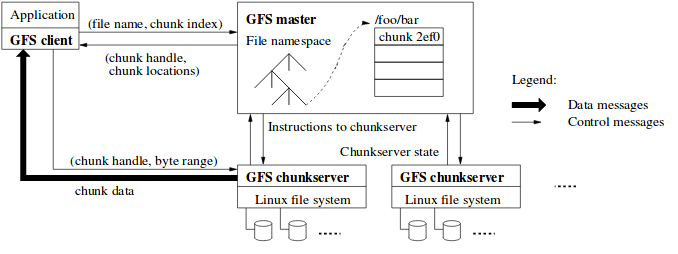
\includegraphics[width=\textwidth]{GFS_Architecture.png}
  \caption{Google File System architecture\cite{Ghem03}}
  \label{GFS_Architecture}
\end{figure}

The GFS architecture that was described in its paper by Google was adapted into an open-source solution called Hadoop \cite{Shv10}. Hadoop was developed mainly by Yahoo!, distributed as an Apache project and functions essentially the same as GFS. There are only minor differences with GFS such as the naming of certain entities and the chunk size. A typical use case of adding a file to the Hadoop File System (HDFS) is show in figure \ref{Hadoop_usecase} below.

\begin{figure}
  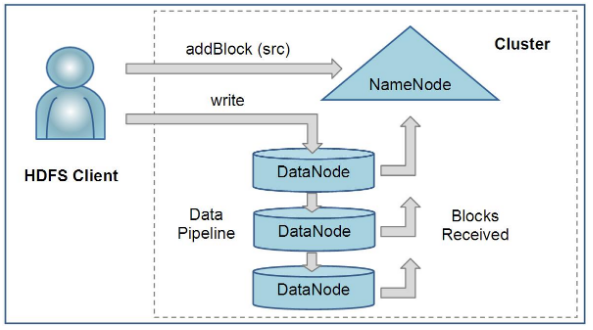
\includegraphics[width=\textwidth]{Hadoop_use_case.png}
  \caption{The data flow when adding a file to the HDFS\cite{Shv10}}
  \label{Hadoop_usecase}
\end{figure}

\paragraph{Uses of the frameworks}
The storage framework highlighted above, is the most-common file-system that empower Big Data implementations today. These implementations are frameworks such as MapReduce and the Apache Spark engine.

\paragraph{MapReduce}
MapReduce is a new framework for processing data and was developed by Google\cite{Dean04} in order to process data in a distributed setting. Firstly, in the \textit{map phase} all data is split into tuples (called key-value pairs). Then, during the shuffle phase, these key-value pairs are shuffled and passed to the \textit{reduce phase} in which a calculation (often an aggregation) is performed on them to generate the a single output value. The main benefit of this framework is that the data can be distributed across a large amount of machines (which are using for example GFS or HDFS). Additionally, instead of communicating the data between the nodes, the program is communicated between the nodes which is magnitudes smaller and more efficient to pass around. A general overview of the execution of a map-reduce problem is given in figure \ref{mapreduce_execution}.

\begin{figure}
  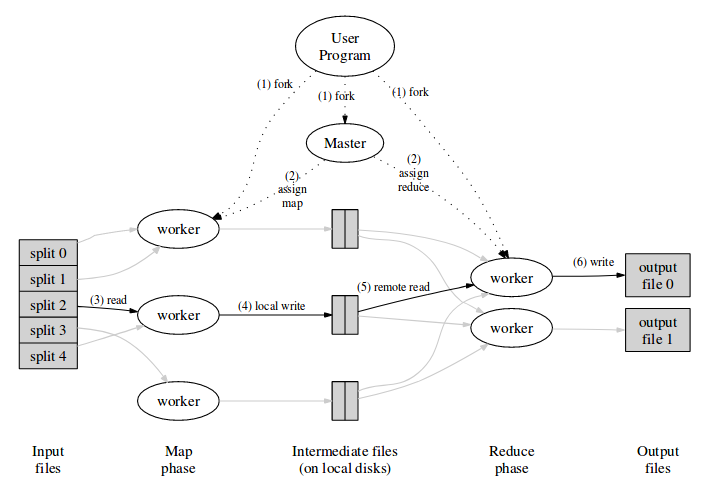
\includegraphics[width=\textwidth]{mapreduce_execution.png}
  \caption{Overview of the execution of a mapreduce problem\cite{Dean04}}
  \label{mapreduce_execution}
\end{figure}

Furthermore the MapReduce framework is similar to the \textit{Bulk-Synchronous processing (BSP)} style which is a little older. However, there are some differences as the MapReduce framework does not allow communication between nodes in the map phase, but only allows communication during the shuffle phase, in-between the mapping and reduce phase\cite{Pace12}.\\
Since BSP and Map-reduce are so similar, peope have worked on transforming BSP tasks into MapReduce tasks. Goodrich et al.\cite{Goo11} has shown that all BSP programs can be converted into MapReduce programs and other researchers have gone as far as to say that all MapReduce task are so similar to BSP tasks that, because BSP has a more theoretical basis, all tasks should be modeled as BSP tasks but implemented using the Map-reduce framework in order to gain the speed of MapReduce and the correctness of BSP\cite{Pace12}.

\paragraph{Apache Spark}
Like MapReduce, Apache Spark is another service built on top of a distributed file system to run programs on a distributed dataset. Spark is an open-source cluster-computing framework that is capable of executing an entire directed acyclic graph of transformations (like mappings) and actions (like reductions) fully in memory\cite{Sparkwebsite}. This is contrast to MapReduce, that forces the programmer to first use a mapping phase and then a reduce phase. This way, Spark is a lot faster than MapReduce because when, for example, 2 mapping phases are needed, 2 MapReduce tasks need to be executed which both require to write all (intermediate) data to the disk. Spark on the other hand can keep all the data in-memory which saves expensive writes to the disk, but needs to take additional steps to prevent losing processed data when there's a power outage.\\

The way in which Spark solves this problem is by using \textbf{RDDs} (Resilient Distributed Datasets). These datasets are read-only and new ones can only be created from data stored on the disk, or transforming existing RDDs\cite{Zaha12}. The Resilient part comes into play when the data is lost. Each RDD has a lineage graph, which shows what transformations have been executed on it. This means that once some data is lost, Spark can trace the path that RDD has followed by using the lineage graph and recalculate any lost data. It is important that the lineage graph does not contain any cycles, i.e. is a Directed Acylic Graph (DAG), because otherwise the data cannot be recovered as Spark will run into an infinite loop.

\begin{figure}
  \begin{center}
    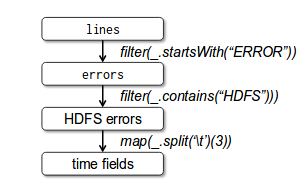
\includegraphics[scale=0.5]{Lineage_graph.png}
  \end{center}
  \caption{Example of the lineage graph of an RDD\cite{Zaha12}}
  \label{lineagegraph}
\end{figure}

\subsubsection{Domain-specific implementations}
\subsubsection{Current challenges}
\paragraph{Performance}

A tradeoff that’s seen frequently is the reduction of wall-clock time at the expense of total processing time (i.e. decreased efficiency). When compute resources are affordable enough, many real-world use cases of machine learning benefit most from being trained rapidly. The fact that this often implies a large multiple in total compute resources (and the associated energy consumption) is not as important, as long as a model saves more money than it costs to run.  A good example of this is found in \citet{DistBelief2012}, where wall clock time speedup factors are achieved by increasing the number of machines quadratically or worse. It still delivered Google competitive advantage for years. Distributed use of GPUs, as in Tensorflow, has better properties, but often still exhibits efficiency below 75\%.
These performance concerns are much less severe in the context of synchronous SGD-based frameworks, which often do achieve linear speedups in benchmarks. However, most of these benchmarks test at most a few hundred machines, whereas the scale at which e.g. DistBelief is demonstrated can sometimes be two orders of magnitude larger. The reason for this is unclear, although it might be related to the fault tolerance concerns mentioned below. Synchronous frameworks also benefit more from high-bandwidth links such as InfiniBand due to the fact that all nodes' communication is synchronized, even though they are expensive (with costs running up to thousands of euros for even a cheap switch) and can't practically be used in large footprint clusters (e.g. in multiple datacenters) due to wiring and latency constraints.

\paragraph{Fault tolerance}

Synchronous AllReduce-based approaches seem to scale significantly better than the parameter server approach (up to a certain cluster size), but suffer from a lack of fault-tolerance: failure of a single machine blocks the entire training process. At smaller scales this might still be a manageable problem, but past a certain number of nodes the probability of any node being unavailable becomes high enough to lead to near-continuous stalling. Common implementations of these HPC-inspired patterns, such as MPI and NCCL, lack fault-tolerance completely, and although there are efforts to counteract some of this, production-ready solutions are lacking. Some of the described implementations allow for checkpointing to counteract this, but a lot of work is necessary to enable true fault-tolerance, such as described in \citet{Amatya2017}. It is also possible to reduce the probability of failure for each individual node, but this requires very specific hardware that is expensive (e.g. highly stable datacenter cooling or Infiniband networks) and not generally available on commodity cloud platforms.
Asynchronous implementations do not suffer from this problem quite as much, as they are designed to explicitly tolerate straggling and failing nodes, with only minimal impact on training performance. The question for ML practitioners, then, is whether they prefer performance or fault tolerance, and whether they are constrained by either one. Hybrid approaches even offer a way to customize these characteristics, although they are not frequently found in use yet. It would be interesting to see whether an even better approach exists, or whether there is an efficient way to implement fault-tolerant AllReduce.

\paragraph{Privacy}

There are scenarios in which it is beneficial or even mandatory to isolate different subsets of the training data from each other. The furthest extent of this is when a model needs to be trained on datasets that each live on different machines/clusters, and may under no circumstance be colocated or even moved.
One interesting approach to training a model in a privacy-sensitive context is the use of a distributed ensemble model. This allows perfect separation of the training data subsets, with the drawback that a method needs to be found to properly balance each trained model's output for an unbiased result.
Parameter server-based systems could also be useful in the context of privacy, as the training of a model can be separated from the training's result. However, this assumes that no sensitive properties of the underlying data leak into the model itself, which is not easy to prove.
Finally, it is possible to introduce statistical noise into each subset of the training data, with the intention of rendering its sensitive characteristics unidentifiable to other parties. \citet{Bal12} touches on this subject, but makes it clear that the amount privacy in this scenario is dependent on the amount of statistical queries required to learn the dataset, which puts an upper bound on the usefulness of the model itself.
In conclusion, it is highly unlikely that perfect privacy is possible, but current frameworks do not offer much support for even basic variants. It could be interesting to answer whether there's a generic way to facilitate distributed privacy, which could then be integrated into the frameworks that are being used.

